\documentclass[openany]{article}

%Typesetting and language
\usepackage[american]{babel}
\usepackage[T1]{fontenc}
\usepackage{charter}
\usepackage{enumitem}
\usepackage{hyperref}

%Symbols
\usepackage{amssymb, amsmath, amsthm, bm}
\usepackage{mathrsfs}
\usepackage{mathtools}
\usepackage{marvosym}
\usepackage{MnSymbol}

%Colors & graphics
\usepackage[dvipsnames]{xcolor}
\usepackage{pgfplots}
\usepackage[numbered,framed]{matlab-prettifier}
\usepackage{pgfplots}
\usepackage{listings}
\usepackage{tikz}
\usetikzlibrary{arrows.meta}
\usepackage[object=vectorian]{pgfornament}
\usepackage{wrapfig}
\usepackage{varwidth}
\usepackage[framemethod=TikZ]{mdframed}
\usepackage{caption}
\usepackage{float}
\usepackage{geometry}
\usepackage{ulem}
\usepackage[most]{tcolorbox}
\usepackage{array}

\setlength{\parindent}{0pt}

\makeatletter
\g@addto@macro\bfseries{\boldmath}
\makeatother


\renewcommand{\Re}{\mathfrak{Re}}
\renewcommand{\Im}{\mathfrak{Im}}

\geometry{left=2cm,right=2cm,bottom=2cm,top=2cm}

\usepackage{fancyhdr}
\pagestyle{fancy}
\fancyhf{}
\renewcommand{\sectionmark}[1]{\markright{\arabic{section} - #1}}
\cfoot{\thepage}
\lhead{Algo Learning}
\chead{Dynamic Programming}
\rhead{Adam Yang}
\renewcommand{\headrulewidth}{1pt}


\DeclareMathOperator{\sgn}{sgn}
\DeclareMathOperator{\im}{im}
\DeclareMathOperator{\var}{var}
\DeclareMathOperator{\Orb}{Orb}
\DeclareMathOperator{\Fix}{Fix}
\DeclareMathOperator{\Stab}{Stab}
\DeclareMathOperator{\cov}{cov}
\DeclareMathOperator*{\esssup}{ess\,sup}
\DeclareMathOperator{\corr}{corr}
\DeclareMathOperator{\lik}{lik}
\DeclareMathOperator*{\argmin}{argmin}
\DeclareMathOperator*{\argmax}{argmax}

\newcommand{\niceline}[2]{%
		\nointerlineskip \vspace{.5\baselineskip}\hspace{\fill}
		{\color{#1}
				\resizebox{0.5\linewidth}{2ex}
				{{%
								{\begin{tikzpicture}
										\node  (C) at (0,0) {};
										\node (D) at (9,0) {};
										\path (C) to [ornament=#2] (D);
										\end{tikzpicture}}}}}%
		\hspace{\fill}
		\par\nointerlineskip \vspace{.5\baselineskip}
}

\definecolor{darkViolet}{HTML}{9400D3}
\newcommand{\sweetline}{%
		\noindent
		\begin{center}
				{\color{darkViolet}
						\resizebox{0.5\linewidth}{1ex}
						{{%
										{
\begin{tikzpicture}
												\node  (C) at (0,0) {};
												\node (D) at (9,0) {};
												\path (C) to [ornament=85] (D);
												\end{tikzpicture}}}}}%
		\end{center}
}

\definecolor{remarkPurple}{HTML}{8346FF}
\definecolor{defBlue}{HTML}{0673FF}
\definecolor{exPurple}{HTML}{FF8710}

%THEOREM
\newtcbtheorem[auto counter,number within=section]{theorem}{Theorem}%
{enhanced,colback=white, breakable,frame empty,interior empty,colframe=cyan!50!white, top=8mm,
				coltitle=black,fonttitle=\bfseries,colbacktitle=cyan!15!white,
				borderline={0.5mm}{0mm}{cyan!15!white},
				borderline={0.5mm}{0mm}{cyan!50!white,dashed},
				attach boxed title to top left={yshift=-4mm},
				boxed title style={sharp corners=east,boxrule=1pt},varwidth boxed title}{thm}

%PROPOSITION
\newtcbtheorem[use counter from=theorem]{proposition}{Proposition}%
{enhanced,colback=white,breakable,frame empty,interior empty,colframe=defBlue!75!white, top=8mm,
				coltitle=black,fonttitle=\bfseries,colbacktitle=defBlue!20!white,
				borderline={0.5mm}{0mm}{defBlue!20!white},
				borderline={0.5mm}{0mm}{defBlue!50!white,dashed},
				attach boxed title to top left={yshift=-4mm},
				boxed title style={sharp corners=east,boxrule=1pt},varwidth boxed title}{prop}

%DEFINITION
\newtcbtheorem[use counter from=theorem]{definition}{Definition}%
{enhanced,colback=white,breakable,frame empty,interior empty,colframe=defBlue!75!white, top=8mm,
				coltitle=black,fonttitle=\bfseries,colbacktitle=defBlue!20!white,
				borderline={0.5mm}{0mm}{defBlue!20!white},
				borderline={0.5mm}{0mm}{defBlue!50!white,dashed},
				attach boxed title to top left={yshift=-4mm},
				boxed title style={sharp corners=east,boxrule=1pt},varwidth boxed title}{def}

%COROLLARY
\newtcbtheorem[use counter from=theorem]{corollary}{Corollary}%
{enhanced,colback=white,breakable,frame empty,interior empty,colframe=defBlue!75!white, top=8mm,
				coltitle=black,fonttitle=\bfseries,colbacktitle=defBlue!20!white,
				borderline={0.5mm}{0mm}{defBlue!20!white},
				borderline={0.5mm}{0mm}{defBlue!50!white,dashed},
				attach boxed title to top left={yshift=-4mm},
				boxed title style={sharp corners=east,boxrule=1pt},varwidth boxed title}{cor}

%REMARK
\newtcbtheorem[no counter]{remark}{Remark}%
{detach title, colback=white,enhanced ,breakable,frame empty, interior empty, fonttitle=\bfseries, coltitle=Violet, before upper={\tcbtitle.\quad},
				borderline west={0.5mm}{0mm}{remarkPurple!40!white},
				borderline west={0.5mm}{0mm}{remarkPurple!60!white,dashed}}{remark}

%LEMMA
\makeatletter
\newtcbtheorem[number within = tcb@cnt@theorem]{lemma}{Lemma}%
{enhanced,breakable,colback=white,frame empty,interior empty,colframe=orange!75!white, top=8mm,
				coltitle=black,fonttitle=\bfseries,colbacktitle=orange!20!white,
				borderline={0.5mm}{0mm}{orange!20!white},
				borderline={0.5mm}{0mm}{orange!50!white,dashed},
				attach boxed title to top left={yshift=-4mm},
				boxed title style={sharp corners=east,boxrule=1pt},varwidth boxed title}{lemma}
\makeatother


%PROOF
%%{enhanced,breakable,frame empty,interior empty,colframe=remarkPurple!75!white, top=8mm,
%	coltitle=black,fonttitle=\bfseries,colbacktitle=remarkPurple!20!white,
%	borderline={0.5mm}{0mm}{remarkPurple!20!white},
%	borderline={0.5mm}{0mm}{remarkPurple!50!white,dashed},
%	attach boxed title to top left={yshift=-4mm},
%	boxed title style={sharp corners=east,boxrule=1pt},varwidth boxed title}{prf}


\tcolorboxenvironment{proof}{% amsthm' 
				blanker,breakable,left=5mm,
				before skip=10pt,after skip=10pt,
				borderline west={0.5mm}{0pt}{cyan!40},
				borderline west={0.5mm}{0pt}{remarkPurple!10, dashed}}

%PROBLEM
\newtcbtheorem[auto counter]{problem}{Problem}%
{enhanced,breakable,colback=white,frame empty,interior empty,colframe=cyan!50!white, top=8mm,
				coltitle=black,fonttitle=\bfseries,colbacktitle=cyan!20!white,
				borderline={0.5mm}{0mm}{cyan!20!white},
				borderline={0.5mm}{0mm}{cyan!50!white,dashed},
				attach boxed title to top left={yshift=-4mm},
				boxed title style={sharp corners=east,boxrule=1pt},varwidth boxed title}{prob}

%EXAMPLE
%\newtcbtheorem[use counter from=problem]{example}{Example}%
%{enhanced,breakable,colback=white,frame empty,interior empty,colframe=remarkPurple!50!white, top=8mm,
%		coltitle=black,fonttitle=\bfseries,colbacktitle=remarkPurple!30!white,
%		borderline={0.5mm}{0mm}{remarkPurple!30!white},
%		borderline={0.5mm}{0mm}{remarkPurple!30!white,dashed},
%		attach boxed title to top left={yshift=-4mm},
%		boxed title style={sharp corners=east,boxrule=1pt},varwidth boxed title}{ex}


\newtcbtheorem[use counter from=theorem]{example}{Example}%
{detach title, colback=white,enhanced ,breakable,frame empty, interior empty, fonttitle=\bfseries, coltitle=black, before upper={\tcbtitle.\quad},
		borderline west={0.5mm}{0mm}{remarkPurple!30!white},
		borderline ={0.5mm}{0mm}{remarkPurple!30!white}}{example}

%SOLUTION
\newtcbtheorem[no counter]{solution}{Solution}%
{enhanced,breakable,colback=white,frame empty,interior empty,colframe=green!75!white, top=8mm,
				coltitle=black,fonttitle=\bfseries,colbacktitle=green!20!white,
				borderline={0.5mm}{0mm}{green!20!white},
				borderline={0.5mm}{0mm}{green!50!white,dashed},
				attach boxed title to top left={yshift=-4mm},
				boxed title style={sharp corners=east,boxrule=1pt},varwidth boxed title}{sol}
\definecolor{realPurple}{HTML}{AA05F9}
\definecolor{gray}{rgb}{0.5,0.5,0.5}
\definecolor{dkgreen}{rgb}{0,0.6,0}
\definecolor{mauve}{rgb}{0.58,0,0.82}

\lstset{frame=tb,
				style=Matlab-editor,
				language=C,
				aboveskip=3mm,
				belowskip=3mm,
				xleftmargin=3mm,
				showstringspaces=false,
				columns=flexible,
				frame=none,
				basicstyle={\small\ttfamily},
				numberstyle=\tiny\color{gray},
				keywordstyle=\color{blue},
				commentstyle=\color{dkgreen},
				stringstyle=\color{mauve},
				breaklines=true,
				breakatwhitespace=true,
				mlshowsectionrules = true,
				tabsize=3,
				backgroundcolor=\color{cyan!5}
}

\newcommand\mmybox[2][fill=cyan!20]{%
    \tikz[baseline]\node[%
        inner ysep=0pt, 
        inner xsep=2pt, 
        anchor=text, 
        rectangle, 
        rounded corners=1mm,
        #1] {\strut#2};%
}


\def\changemargin#1#2{\list{}{\rightmargin#2\leftmargin#1}\item[]}
\let\endchangemargin=\endlist

\linespread{1.4}



% MAIN DOC
\begin{document}

\title{Dynamic Programming}
\author{Adam Yang}
% \date{\today}
\maketitle


\begin{definition*}{High Level Understanding}
    One way to think about it: avoid duplicating work in backtracking solutions (when it is possible).

    Closely related to recursive thinking: What smaller problems do I need to have solved to be able to now solve a bigger problem?

    Contrast to Greedy: What is our first step? Commit to it, then solve a new problem.
\end{definition*}

\subsection*{Warm-Up}

\begin{problem*}{}
    Find the n-th Fib Number
\end{problem*}
\begin{solution*}{recursive, not optimal}
            Let $f(n)$ be the n-th fib number, we have
        
	\[f(0)=f(1)=1\]
        \[n\geq 2: f(n)=f(n-1)+f(n-2)\]
        \[T(n)=T(n-1)+T(n-2)+O(1)\]

        So $T(n)\geq f(n)$, which grows roughly as Golden-Ratio.
        
        Golden Ratio is the $x$ solving $x^2=x+1, x\approx 1.618$. The running time is exponential.
\end{solution*}
		% \renewcommand{\qedsymbol}{} % hide the QED square



 \begin{proof}[Improvement]{}
        		\renewcommand{\qedsymbol}{} % hide the QED square
                This recalculates $f(n-2)$ twice, and as a result, recalculates $f(n-3)$ for more often, and so on. We should instead store the result once we have computed it. At that point, we get rid of recursion:

        \qquad \texttt{int Fib[n+1];}\texttt{}
        
        \qquad \texttt{Fib[0] = Fib[1] = 1;}
        
        \qquad \texttt{for(int i=2; i $\leq$ n; ++i) Fib[i]=Fib[i-1]+Fib[i-2];}

        This makes the running time to $O(n)$
        \end{proof}
% unnumbered theorem/proposition/definition/example/etc: add *

\begin{problem*}{Weighted Interval Selection}
    Same as our original selection problem:
    $n$ intervals with start times s(i), finish time f(i), and \textbf{*weights*} w(i).

    \textbf{Goal:} select a set S of intervals where no two intervals overlap, and so that the total weight of selected intervals is maximized.

    \textbf{Application:} weights could be importance/interest of events between which we need to choose
\end{problem*}

\begin{proof}[Analysis]{}
		\renewcommand{\qedsymbol}{} % hide the QED square
        Greedy gives us suboptimal solution. \textbf{No greedy rule will work}
\end{proof}
\begin{proof}[Key Insight:]{}
		\renewcommand{\qedsymbol}{} % hide the QED square
        Exhaustive search works, but the running time is $2^n$. 

        If we have intervals 1, ..., n available, the pimum solution for those intervals does one of the following (with respect to interval $i$):

        \qquad 1) Not include $i$, and get the optimum solution for aol intervals except $i$.
        
        \qquad 2) Include $i$, and get the optimum solution for all intervals except those intersecting $i$, plus the weight that it gets from $i$ itself.

        \qquad Among these, the optimum solution (being optimal) chooses the better one.

        What makes this tick is that once we commit to including $i$, or to not including $i$, we compute/use the \textbf{*optimum*} solution for the resulting subproblem. \textbf{This is the key property for DP:} The optimal solution for a big input contains as subparts the optimal solutions for smaller problems.
\end{proof}



% END MAIN Doc


\begin{theorem*}{Weak Law of Large Numbers}{}
		Let $X_1,X_2,...$ be i.i.d. In order that there exists $\{\mu_n\}$ such that $S_n /n\to \mu_n$ in probability, it is necessary and sufficient that
		\[
				x \mathbb{P}(\lvert X_1\rvert >x) \to 0 \qquad \text{ as }\qquad x\to \infty.
		\] 
		If so, $\mu_n:= \mathbb{E}[X_1 1_{\{\lvert X_1\rvert \leqslant n\}}]$ works.
\end{theorem*}

% idk why each environment is followed by two extra {}{}
% to change theorem's names (or def/proposition/example/etc, basically everything but proofs), enter something in the second {} as shown above
% if only used for homework, it's okay to just * every theorem environment
% to chance the name of a proof, however, replace second {} by [] with text inside. See below
\begin{proof}[Not a proof]{}
		No, this is not the WLLN I know.
\end{proof}

% default proof
\begin{proof}{}{}
		The sufficiency part follows by (i) truncating the variables, (ii) showing truncation has bounded effect, (iii) proving theorem works for truncated variables, and (iv) combining (ii) and (iii) to obtain result.
\end{proof}


\subsection*{Problem -25565} % I use * to suppress automatic numbering except when I write big comprehensive notes

% solution: two versions

\begin{solution*}{}{}
		I don't like this box but you can configure it yourself.
\end{solution*}

\begin{proof}[Solution]{}
		\renewcommand{\qedsymbol}{} % hide the QED square
		Alternatively, this is a ``solution'' environment borrowed from the proof environment. 
\end{proof}

\begin{problem*}{}{}
		Write a function to compute the square root of a \texttt{float}.
\end{problem*}

\begin{proof}[Solution]{}
		\renewcommand{\qedsymbol}{}
		(I don't like to \verb|\usepackage{algorithms}|, so below is an alternative.) 
		\begin{lstlisting}[basicstyle=\fontsize{8}{9}\selectfont\ttfamily]
float Q_rsqrt( float number )
{
	long i;
	float x2, y;
	const float threehalfs = 1.5F;

	x2 = number * 0.5F;
	y  = number;
	i  = * ( long * ) &y;                       // evil floating point bit level hacking
	i  = 0x5f3759df - ( i >> 1 );               // what the fuck? 
	y  = * ( float * ) &i;
	y  = y * ( threehalfs - ( x2 * y * y ) );   // 1st iteration
//	y  = y * ( threehalfs - ( x2 * y * y ) );   // 2nd iteration, this can be removed
	return y;
}
		\end{lstlisting} 
		Convince yourself it works.
\end{proof}

\textbf{Bold} \textit{italic} \emph{underline} \verb|code| and \texttt{more code} \textsc{whatever this is} {\color{cyan} blue/cyan} {\color{red} red} $\mathcal{AND}$ $\mathbb{SO}$ $\mathfrak{ON}$.

\subsection*{\texttt{Tikz} Code for HW3 1a}

\begin{center}
				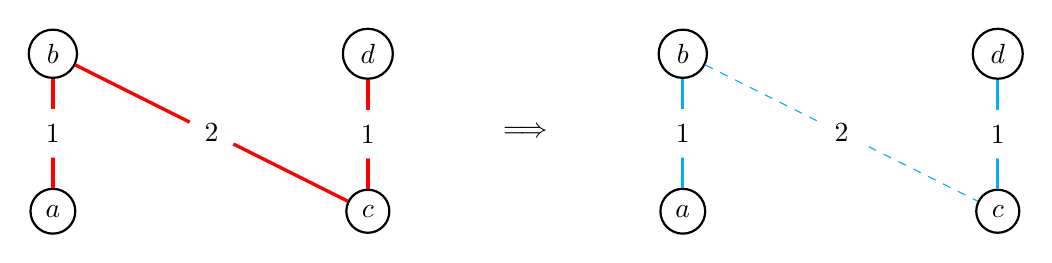
\begin{tikzpicture}
						\begin{scope}[every node/.style={circle,thick,draw}]
								\node (A) at (0,-2) {$a$};
								\node (B) at (0,0) {$b$};
								\node (C) at (4,-2) {$c$};
								\node (D) at (4,0) {$d$};
								\node (A2) at (8,-2) {$a$};
								\node (B2) at (8,0) {$b$};
								\node (C2) at (12,-2) {$c$};
								\node (D2) at (12,0) {$d$};
						\end{scope}
						\node at (6, -1) {$\implies$};
						\begin{scope}[>={Stealth[black]},
										every node/.style={fill=white,circle},
								every edge/.style={draw=red,very thick}]
								\path (A) edge node {$1$} (B);
								\path (B) edge node {$2$} (C);
								\path (C) edge node {$1$} (D);
						\end{scope}
						\begin{scope}[>={Stealth[black]},
										every node/.style={fill=white,circle},
								every edge/.style={draw=cyan,very thick}]
								\path (A2) edge node {$1$} (B2);
								\path (C2) edge node {$1$} (D2);
						\end{scope}
						\begin{scope}[>={Stealth[black]},
										every node/.style={fill=white,circle},
								every edge/.style={draw=cyan, dashed}]
								\path (B2) edge node {$2$} (C2);
						\end{scope}
				\end{tikzpicture}
		\end{center}

\end{document}
